\documentclass[a4paper,11pt,fleqn,twoside,notitlepage]{report}
\usepackage[]{graphicx}\usepackage[]{color}
%% maxwidth is the original width if it is less than linewidth
%% otherwise use linewidth (to make sure the graphics do not exceed the margin)
\makeatletter
\def\maxwidth{ %
  \ifdim\Gin@nat@width>\linewidth
    \linewidth
  \else
    \Gin@nat@width
  \fi
}
\makeatother

\definecolor{fgcolor}{rgb}{0.345, 0.345, 0.345}
\newcommand{\hlnum}[1]{\textcolor[rgb]{0.686,0.059,0.569}{#1}}%
\newcommand{\hlstr}[1]{\textcolor[rgb]{0.192,0.494,0.8}{#1}}%
\newcommand{\hlcom}[1]{\textcolor[rgb]{0.678,0.584,0.686}{\textit{#1}}}%
\newcommand{\hlopt}[1]{\textcolor[rgb]{0,0,0}{#1}}%
\newcommand{\hlstd}[1]{\textcolor[rgb]{0.345,0.345,0.345}{#1}}%
\newcommand{\hlkwa}[1]{\textcolor[rgb]{0.161,0.373,0.58}{\textbf{#1}}}%
\newcommand{\hlkwb}[1]{\textcolor[rgb]{0.69,0.353,0.396}{#1}}%
\newcommand{\hlkwc}[1]{\textcolor[rgb]{0.333,0.667,0.333}{#1}}%
\newcommand{\hlkwd}[1]{\textcolor[rgb]{0.737,0.353,0.396}{\textbf{#1}}}%

\usepackage{framed}
\makeatletter
\newenvironment{kframe}{%
 \def\at@end@of@kframe{}%
 \ifinner\ifhmode%
  \def\at@end@of@kframe{\end{minipage}}%
  \begin{minipage}{\columnwidth}%
 \fi\fi%
 \def\FrameCommand##1{\hskip\@totalleftmargin \hskip-\fboxsep
 \colorbox{shadecolor}{##1}\hskip-\fboxsep
     % There is no \\@totalrightmargin, so:
     \hskip-\linewidth \hskip-\@totalleftmargin \hskip\columnwidth}%
 \MakeFramed {\advance\hsize-\width
   \@totalleftmargin\z@ \linewidth\hsize
   \@setminipage}}%
 {\par\unskip\endMakeFramed%
 \at@end@of@kframe}
\makeatother

\definecolor{shadecolor}{rgb}{.97, .97, .97}
\definecolor{messagecolor}{rgb}{0, 0, 0}
\definecolor{warningcolor}{rgb}{1, 0, 1}
\definecolor{errorcolor}{rgb}{1, 0, 0}
\newenvironment{knitrout}{}{} % an empty environment to be redefined in TeX

\usepackage{alltt}
\newcommand{\SweaveOpts}[1]{}  % do not interfere with LaTeX
\newcommand{\SweaveInput}[1]{} % because they are not real TeX commands
\newcommand{\Sexpr}[1]{}       % will only be parsed by R


\setcounter{tocdepth}{3}
\setcounter{secnumdepth}{3}

\usepackage[utf8]{inputenc}
\usepackage[margin=2.5cm]{geometry}
\usepackage{graphicx}
\usepackage[T1]{fontenc}
\usepackage{enumitem}
\usepackage[section]{placeins}
\usepackage{csquotes}
\usepackage[english]{babel}
\usepackage{float}
\usepackage{caption}
\usepackage{makecell}
\usepackage{hyperref}
\usepackage{bm}
\usepackage{newfloat}
\usepackage[linesnumbered,lined,boxed,commentsnumbered]{algorithm2e}
\usepackage{booktabs}
\usepackage{colortbl}
\usepackage{tikz}

\usepackage{amssymb,amsmath,amsthm,amsfonts}
\newtheorem{theorem}{Theorem}

\usepackage{fancyhdr}
\setlength{\headheight}{15pt}

\pagestyle{fancy}
\renewcommand{\chaptermark}[1]{ \markboth{#1}{} }
\renewcommand{\sectionmark}[1]{ \markright{#1}{} }

\fancyhf{}
\fancyfoot[CE,CO]{\thepage}
\fancyhead[LE]{\textit{ \nouppercase{\leftmark}} }
\fancyhead[LO]{\textit{ \nouppercase{\rightmark}} }
%\fancyhead[RE,RO]{Erik Thors\'{e}n, \href{mailto:Ethorsn@gmail.com}{Ethorsn@gmail.com} }
\fancypagestyle{plain}{ %
\fancyhf{} % remove everything
  \renewcommand{\headrulewidth}{0pt} % remove lines as well
  \renewcommand{\footrulewidth}{0pt}
}

\usepackage[citestyle=authoryear,bibstyle=authoryear,natbib=true,backend=bibtex,hyperref=true,maxnames=2]{biblatex}

\bibliography{REFERENCES.bib}

\title{Statistical process control in next-generation sequencing quality control data}
\author{Erik Thors\'{e}n \thanks{Postal adress: Mathematical Statistics, Stockholm University, SE-106 91, Sweden. E-mail: Ethorsn@gmail.com. Supervisors: Taras Bodnar and Johan Dahlberg}}
\date{\today}

\raggedbottom


\begin{document}

\begin{knitrout}
\definecolor{shadecolor}{rgb}{0.969, 0.969, 0.969}\color{fgcolor}\begin{kframe}


{\ttfamily\noindent\itshape\color{messagecolor}{\#\# \\\#\# Attaching package: 'dplyr'}}

{\ttfamily\noindent\itshape\color{messagecolor}{\#\# The following objects are masked from 'package:lubridate':\\\#\# \\\#\#\ \ \ \  intersect, setdiff, union}}

{\ttfamily\noindent\itshape\color{messagecolor}{\#\# The following object is masked from 'package:GGally':\\\#\# \\\#\#\ \ \ \  nasa}}

{\ttfamily\noindent\itshape\color{messagecolor}{\#\# The following objects are masked from 'package:stats':\\\#\# \\\#\#\ \ \ \  filter, lag}}

{\ttfamily\noindent\itshape\color{messagecolor}{\#\# The following objects are masked from 'package:base':\\\#\# \\\#\#\ \ \ \  intersect, setdiff, setequal, union}}

{\ttfamily\noindent\itshape\color{messagecolor}{\#\# Loading required package: parallel}}\end{kframe}
\end{knitrout}

\begin{knitrout}
\definecolor{shadecolor}{rgb}{0.969, 0.969, 0.969}\color{fgcolor}\begin{kframe}
\begin{alltt}
\hlstd{N} \hlkwb{<-} \hlkwd{unique}\hlstd{(df.sample.results}\hlopt{$}\hlstd{flowcell_id)} \hlopt \hlkwd{length}\hlstd{()}
\hlstd{First.date} \hlkwb{<-} \hlkwd{first}\hlstd{(df.sample.results}\hlopt{$}\hlstd{Date)}
\hlstd{last.date} \hlkwb{<-} \hlkwd{last}\hlstd{(df.sample.results}\hlopt{$}\hlstd{Date)}
\end{alltt}
\end{kframe}
\end{knitrout}
In this section we will conduct a exploratory data analysis. We will first introduce the datasets which will be used in this thesis and then continue with exploring them seperately. We will focus our attention to the data of one of each model. 

The data to be used in this thesis consists of two sets. The first set contains observations on the lowest level, what we called tag level. There is no fixed number of tags for each run and therefore each flowcell can contain a different number of measurements. In the tag level dataset, there are a total of $786$ runs (unique flowcells) which have been performed since 2012 up until the end of 2015. 
\begin{knitrout}
\definecolor{shadecolor}{rgb}{0.969, 0.969, 0.969}\color{fgcolor}\begin{kframe}
\begin{alltt}
\hlcom{# Number of flowcells}
\hlstd{N2} \hlkwb{<-} \hlkwd{unique}\hlstd{(All.df.reduced}\hlopt{$}\hlstd{flowcell_id)} \hlopt \hlkwd{length}\hlstd{()}
\hlkwd{rm}\hlstd{(All.df)}
\hlstd{Missing} \hlkwb{<-} \hlkwd{anti_join}\hlstd{(All.df.reduced,df.sample.results,} \hlkwc{by}\hlstd{=}\hlstr{"flowcell_id"}\hlstd{)} \hlopt \hlstd{.}\hlopt{$}\hlstd{flowcell_id} \hlopt \hlkwd{unique}\hlstd{()} \hlopt \hlkwd{length}\hlstd{()}

\hlcom{# exclude data before 2013.}
\hlstd{df.sample.results} \hlkwb{<-} \hlkwd{filter}\hlstd{(df.sample.results,} \hlkwd{year}\hlstd{(Date)}\hlopt{>}\hlnum{2012}\hlstd{)}
\hlstd{All.df.reduced} \hlkwb{<-} \hlkwd{filter}\hlstd{(All.df.reduced,}\hlkwd{year}\hlstd{(Date)}\hlopt{>}\hlnum{2012}\hlstd{)}
\end{alltt}
\end{kframe}
\end{knitrout}
The second dataset contains observations from what we called read level. There are a total of $801$ runs which implies that there is a difference between the datasets. A total of $15$ runs are missing from the Tag level. The missing runs are from the MiSeq 1, HiSeq 3 and 6 machines. These missing runs will be excluded from the data. Also, runs performed in 2012 was done so under different circumstances. It was advised that data from 2012 was not to be used. Therefore, quality control data from 2012 will be removed from our data set.

In Table \ref{CompCycl} we can see the completed run cycles for the HiSeq (Hi) and HiSeqX (HiX) machines. We can start with noticing that HiSeq 1 and 2 are not present in the table. These have been taken out of production. The HiSeqX machines have all been run on the same cycle setting, with every completed cycle equal to 150. This is the only setting used at the SNP\&SEQ platform for HiSeqX. The HiSeq machines shows a much wider range of completed cycles. This is a consequence of the wide range of settings that have been used. We can see that HiSeq 6 (Hi6) have most runs in the vicinity of 124-125 completed cycles. A cycle setting of 126 is one of the most common cycle settings for HiSeq machines at the SNP\&SEQ platform. We will use this machine to represent the HiSeq machines. As the HiSeqX machines did not differ much in the run number we will use the HiSeqX 1 to represent the HiSeqX machines. The MiSeq 1 machine was removed to shorten the table but will be included in further exploratory analysis. It has a wide range of 0-500 completed cycles with a lot of different run settings. Those observations having 0 completed cycles are runs which have been documented to be malfunctions.

The last row in Table \ref{CompCycl} shows the total number of runs performed on each machine. The HiSeq 4 machine has most runs of all but also a large diversity in the run settings. 
\begin{kframe}
\begin{alltt}
\hlcom{# These transformations are to create the table containing the number of flowcells on a specific completed run cycle.}
\hlstd{ggplot.tmp} \hlkwb{<-} \hlstd{df.sample.results[df.sample.results}\hlopt{$}\hlstd{Instrument} \hlopt{!=} \hlstr{"MiSeq 1"}\hlstd{,]} \hlopt
  \hlkwd{group_by}\hlstd{(Instrument,cycles)} \hlopt
  \hlkwd{summarise}\hlstd{(}\hlkwc{x}\hlstd{=}\hlkwd{length}\hlstd{(}\hlkwd{unique}\hlstd{(flowcell_id)))}

\hlstd{ggplot.tmp}\hlopt{$}\hlstd{cycles} \hlkwb{<-} \hlkwd{as.factor}\hlstd{(ggplot.tmp}\hlopt{$}\hlstd{cycles)}

\hlkwd{library}\hlstd{(xtable)}
\hlstd{xtab} \hlkwb{<-} \hlkwd{spread}\hlstd{(ggplot.tmp,}\hlkwc{key}\hlstd{=}\hlstr{"Instrument"}\hlstd{,}\hlkwc{value}\hlstd{=x)}
\hlkwd{colnames}\hlstd{(xtab)} \hlkwb{<-} \hlkwd{c}\hlstd{(}\hlstr{"cycles"}\hlstd{,} \hlkwd{paste0}\hlstd{(}\hlstr{"Hi"}\hlstd{,}\hlnum{3}\hlopt{:}\hlnum{6}\hlstd{),} \hlkwd{paste0}\hlstd{(}\hlstr{"HiX"}\hlstd{,}\hlnum{1}\hlopt{:}\hlnum{5}\hlstd{))}

\hlstd{xtab} \hlkwb{<-} \hlkwd{rbind}\hlstd{(xtab,}\hlkwd{c}\hlstd{(}\hlstr{"NA"}\hlstd{,}\hlkwd{apply}\hlstd{(xtab[,}\hlopt{-}\hlnum{1}\hlstd{],}\hlnum{2}\hlstd{,sum,}\hlkwc{na.rm}\hlstd{=}\hlnum{TRUE}\hlstd{)))}

\hlkwd{print}\hlstd{(}
  \hlkwd{xtable}\hlstd{(xtab,}
         \hlkwc{caption} \hlstd{=} \hlstr{"Table showing the number of completed cycles for each HiSeq (Hi) and HiSeqX (HiX) machine. Notice that the MiSeq 1 machine is removed."}\hlstd{,}
         \hlkwc{label}\hlstd{=}\hlstr{"CompCycl"}\hlstd{),}
  \hlkwc{include.rownames}\hlstd{=}\hlnum{FALSE}\hlstd{)}
\hlcom{# To add last line (below \textbackslash{}hline) I manually used the code generated by the table above.}
\end{alltt}
\end{kframe}
% latex table generated in R 3.2.3 by xtable 1.8-2 package
% Tue Mar  1 09:34:31 2016
\begin{table}[!htb]
\centering
\caption{Table showing the number of flowcells with a specific number of completed cycles for HiSeq (Hi) and HiSeqX (HiX) machine.} 
\begin{tabular}{lccccccccc}
  \toprule 
  & \multicolumn{9}{c}{Machine} \\ \cmidrule(r){2-10} 
cycles & Hi3 & Hi4 & Hi5 & Hi6 & HiX1 & HiX2 & HiX3 & HiX4 & HiX5 \\ 
  \midrule
49 & 7 &  &  &  &  &  &  &  &  \\ 
  50 & 16 & 10 & 11 & 7 &  &  &  &  &  \\ 
  60 &  &  &  & 3 &  &  &  &  &  \\ 
  99 & 2 & 4 & 2 & 1 &  &  &  &  &  \\ 
  100 & 73 & 49 & 15 & 6 &  &  &  &  &  \\ 
  124 &  & 22 & 22 & 30 &  &  &  &  &  \\ 
  125 &  & 53 & 46 & 50 &  &  &  &  &  \\ 
  150 & 11 & 2 & 14 & 16 & 30 & 27 & 22 & 32 & 16 \\ 
  200 &  &  &  & 1 &  &  &  &  &  \\ 
  250 & 6 & 1 &  &  &  &  &  &  &  \\ 
  \midrule
  $\Sigma$ & 115 & 141 & 110 & 114 & 30 & 27 & 22 & 32 & 16 \\ 
   \bottomrule
\end{tabular}
\label{CompCycl}
\end{table}

We will now investigate investigate the mean q values of each successive run at a tag level. In Figure \ref{fig:TagLevelTS} we can see the mean of lane 1 mean q tag level measurements together with the range (min to max) for three different machines of different types. The observations are presented in their order of appearance.

The HiSeq 6 machine shows that some runs has at least one tag level mean Q equal to zero. The variability inside read 2 is larger compared to measurements made in on read 1. The variablility is larger for HiSeq 6 and Miseq 1 machines compared to HiSeqX. At some occasions the range is large in read 2 while not showing the same behaviour in read 1. The MiSeq 1 machine shows much more variation overall, which was to be expected since the MiSeq machine was used for experimental samples on several different settings. 
\begin{knitrout}
\definecolor{shadecolor}{rgb}{0.969, 0.969, 0.969}\color{fgcolor}\begin{kframe}
\begin{alltt}
\hlcom{# Create data.frame containing mean and range of mean q measurements on tag level}
\hlstd{ggplot.tmp1} \hlkwb{<-} \hlstd{df.sample.results} \hlopt
  \hlkwd{filter}\hlstd{(Instrument} \hlopt{==} \hlstr{"HiSeq 6"} \hlopt{|}
         \hlstd{Instrument} \hlopt{==} \hlstr{"MiSeq 1"} \hlopt{|}
         \hlstd{Instrument} \hlopt{==} \hlstr{"HiSeqX 1"}\hlstd{,}
         \hlstd{lane_num} \hlopt{==} \hlnum{1}\hlstd{)} \hlopt
  \hlkwd{group_by}\hlstd{(Date,flowcell_id, Instrument, read_num)} \hlopt
  \hlkwd{summarise}\hlstd{(}\hlkwc{mn} \hlstd{=} \hlkwd{mean}\hlstd{(mean_q),} \hlkwc{min} \hlstd{=} \hlkwd{min}\hlstd{(mean_q),} \hlkwc{max} \hlstd{=} \hlkwd{max}\hlstd{(mean_q))} \hlopt
  \hlkwd{group_by}\hlstd{()} \hlopt
  \hlkwd{arrange}\hlstd{(}\hlkwd{desc}\hlstd{(Instrument))}
\hlcom{# How many observations for each machine?}
\hlstd{n1} \hlkwb{<-} \hlkwd{filter}\hlstd{(ggplot.tmp1, Instrument} \hlopt{==} \hlstr{"HiSeq 6"}\hlstd{)} \hlopt \hlkwd{nrow}\hlstd{()}
\hlstd{n2} \hlkwb{<-} \hlkwd{filter}\hlstd{(ggplot.tmp1, Instrument} \hlopt{==} \hlstr{"HiSeqX 1"}\hlstd{)} \hlopt \hlkwd{nrow}\hlstd{()}
\hlstd{n3} \hlkwb{<-} \hlkwd{filter}\hlstd{(ggplot.tmp1, Instrument} \hlopt{==} \hlstr{"MiSeq 1"}\hlstd{)} \hlopt \hlkwd{nrow}\hlstd{()}

\hlcom{# Order of appearance: MiSeq 1, HiSeqX 1, HiSeq 6  }
\hlstd{OrderOfApp} \hlkwb{<-} \hlkwd{c}\hlstd{(}\hlkwd{rep}\hlstd{(}\hlkwd{seq}\hlstd{(}\hlnum{1}\hlstd{,n3}\hlopt{/}\hlnum{2}\hlstd{,} \hlkwc{by}\hlstd{=}\hlnum{1}\hlstd{),} \hlkwc{each}\hlstd{=}\hlnum{2}\hlstd{),} \hlkwd{rep}\hlstd{(}\hlkwd{seq}\hlstd{(}\hlnum{1}\hlstd{,n2}\hlopt{/}\hlnum{2}\hlstd{,} \hlkwc{by}\hlstd{=}\hlnum{1}\hlstd{),}\hlkwc{each}\hlstd{=}\hlnum{2}\hlstd{),} \hlkwd{rep}\hlstd{(}\hlkwd{seq}\hlstd{(}\hlnum{1}\hlstd{,n1}\hlopt{/}\hlnum{2}\hlstd{,} \hlkwc{by}\hlstd{=}\hlnum{1}\hlstd{),}\hlkwc{each}\hlstd{=}\hlnum{2}\hlstd{))}
\hlcom{# Mutate Date to order of appearance.}
\hlstd{ggplot.tmp1} \hlkwb{<-} \hlkwd{mutate}\hlstd{(ggplot.tmp1,} \hlkwc{Date} \hlstd{= OrderOfApp)}
\hlcom{# Rename variables for nicer printing}
\hlstd{ggplot.tmp1} \hlkwb{<-} \hlkwd{rename}\hlstd{(ggplot.tmp1,} \hlkwc{Machine}\hlstd{=Instrument,} \hlkwc{Read}\hlstd{=read_num)}
\hlcom{# Create figure of mean and range of mean q measurements on tag level}
\hlkwd{ggplot}\hlstd{(ggplot.tmp1,}
       \hlkwd{aes}\hlstd{(}\hlkwc{x}\hlstd{=Date,}\hlkwc{y}\hlstd{=mn))} \hlopt{+}
  \hlkwd{geom_errorbar}\hlstd{(}\hlkwd{aes}\hlstd{(}\hlkwc{ymin}\hlstd{=min,}
                    \hlkwc{ymax}\hlstd{=max,}
                    \hlkwc{color}\hlstd{=}\hlstr{"#7fcdbb"}\hlstd{),}
                \hlkwc{stat}\hlstd{=}\hlstr{"identity"}\hlstd{,}
                \hlkwc{width}\hlstd{=}\hlnum{0.5}\hlstd{,}
                \hlkwc{alpha}\hlstd{=}\hlnum{0.8}\hlstd{)} \hlopt{+}
  \hlkwd{scale_shape_identity}\hlstd{()} \hlopt{+}
  \hlkwd{geom_point}\hlstd{(}\hlkwd{aes}\hlstd{(}\hlkwc{color}\hlstd{=}\hlstr{"#990000"}\hlstd{),} \hlkwc{alpha}\hlstd{=}\hlnum{0.6}\hlstd{)} \hlopt{+}
  \hlkwd{facet_grid}\hlstd{(Read}\hlopt{~}\hlstd{Machine,}
             \hlkwc{scales} \hlstd{=} \hlstr{"free"}\hlstd{,}
             \hlcom{#ncol=2,}
             \hlkwc{labeller} \hlstd{= label_both)} \hlopt{+}
  \hlkwd{theme_bw}\hlstd{()} \hlopt{+}
  \hlkwd{ylab}\hlstd{(}\hlstr{"value"}\hlstd{)} \hlopt{+}
  \hlkwd{scale_color_manual}\hlstd{(}\hlstr{""}\hlstd{,}
                     \hlkwc{label}\hlstd{=}\hlkwd{c}\hlstd{(}\hlstr{"Range (min-max)"}\hlstd{,}\hlstr{"mean"}\hlstd{),}
                     \hlkwc{values}\hlstd{=}\hlkwd{c}\hlstd{(}\hlstr{"#7fcdbb"}\hlstd{,}\hlstr{"#990000"}\hlstd{))} \hlopt{+}
  \hlkwd{theme}\hlstd{(}\hlkwc{axis.text.x}\hlstd{=}\hlkwd{element_text}\hlstd{(}\hlkwc{angle}\hlstd{=}\hlnum{60}\hlstd{,}
                                 \hlkwc{vjust}\hlstd{=}\hlnum{0.7}\hlstd{,}
                                 \hlkwc{hjust}\hlstd{=}\hlnum{0.8}\hlstd{),}
        \hlkwc{legend.position}\hlstd{=}\hlstr{"bottom"}\hlstd{)} \hlopt{+}
  \hlkwd{guides}\hlstd{(}\hlkwc{color}\hlstd{=}\hlkwd{guide_legend}\hlstd{(}\hlkwc{override.aes}\hlstd{=}\hlkwd{list}\hlstd{(}\hlkwc{shape}\hlstd{=}\hlkwd{c}\hlstd{(}\hlnum{NA}\hlstd{,}\hlnum{16}\hlstd{),}\hlkwc{linetype}\hlstd{=}\hlkwd{c}\hlstd{(}\hlnum{1}\hlstd{,}\hlnum{0}\hlstd{))))}\hlopt{+}
  \hlkwd{ggtitle}\hlstd{(}\hlstr{"mean-Q score measurements on Tag level"}\hlstd{)} \hlopt{+}
  \hlkwd{xlab}\hlstd{(}\hlstr{"Order of appearance"}\hlstd{)}
\end{alltt}
\end{kframe}\begin{figure}[!htb]
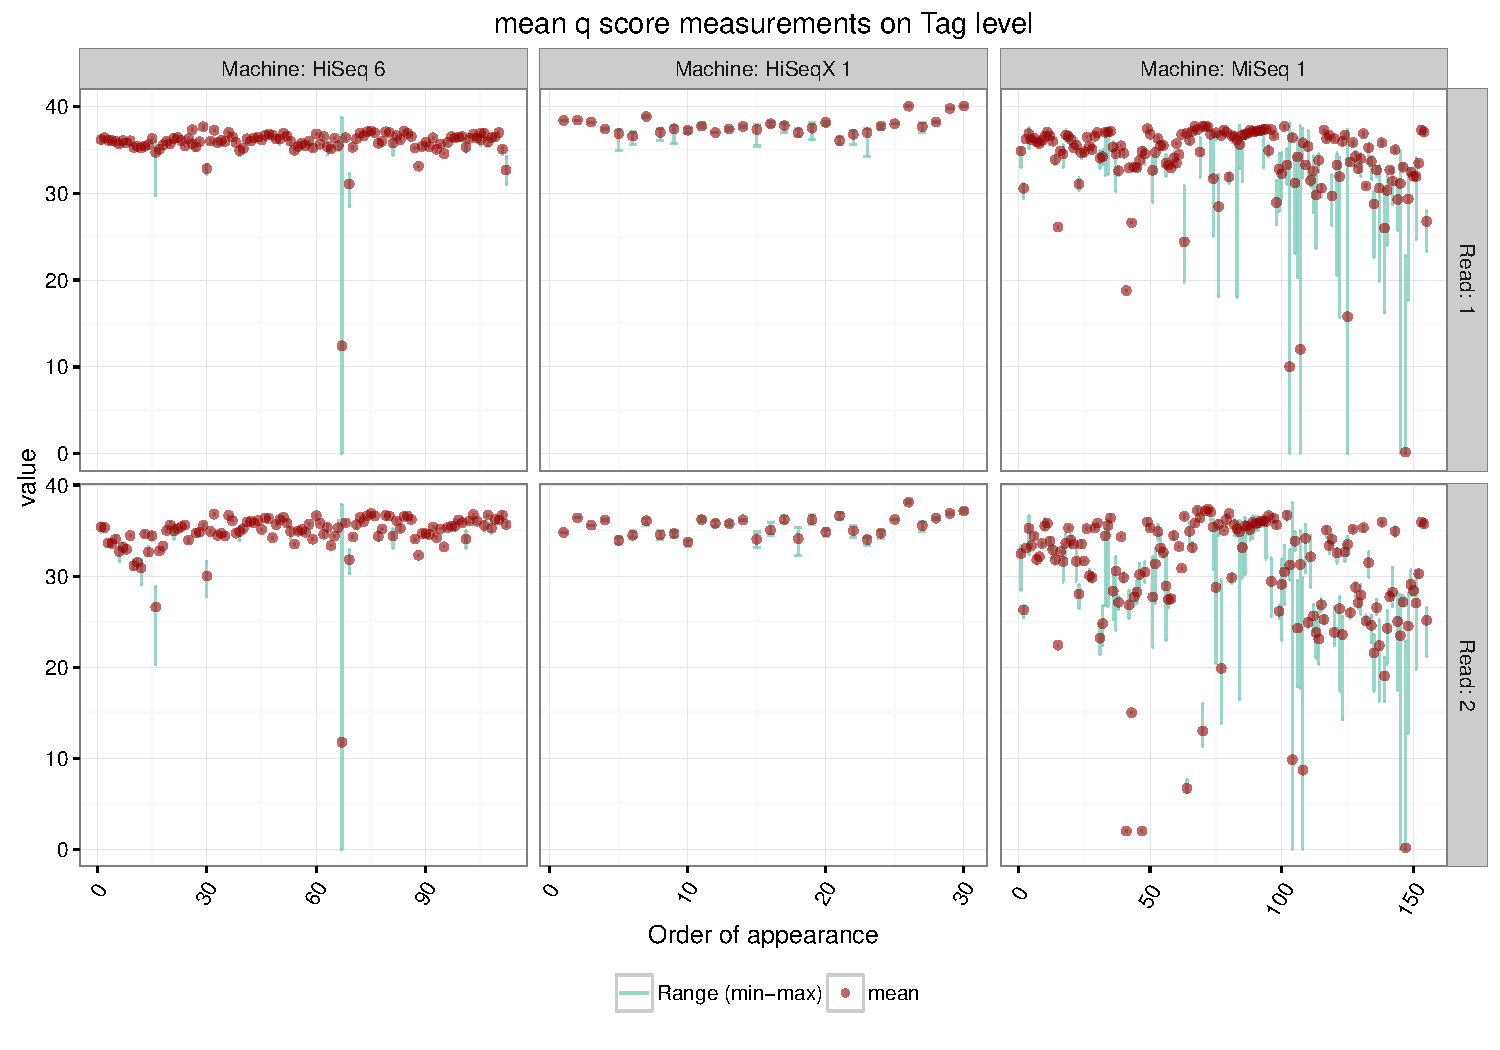
\includegraphics[width=\maxwidth]{figure/TagLevelTS-1} \caption[Figure containing the range (min to max) and mean of each successive run (flowcell)]{Figure containing the range (min to max) and mean of each successive run (flowcell). Here, we are showing read 1 and 2 in lane 1, disregarding what type of setting the run is performed on.}\label{fig:TagLevelTS}
\end{figure}


\end{knitrout}
We will now focus on the HiSeq 6 machine with 102 to 126 completed cycles, in order to make this EDA sufficiently short. 

In Figure \ref{fig:HiSeq6Comb} the range together with the mean of lane 1 and read 1 is shown in their order of appearance. The variables shown here are percent data above a q-score of 30 and the percent tag error. These measurements are from tag level for the HiSeq 6 machine with a cycle setting of 102 to 126. The last figure contains the number of observations in each lane 1 and read 1. %Also, the scale of the percentage is reversed such that both variables graphical interpretation are the same. A low value is not desirable. 
The first variable, the percentage of data above a Q score of 30, which we will refer to as percent Q30, shows a overall small amount of variation. When the spread increases the mean does aswell. The percent tag error can be seen to be very close to zero and at some times equal to zero. This is surprising since the construction of the variable is connected to the error rate. If one is zero, the other should be aswell. However, for \textit{some} runs with zero percent tag error, the error rate is well above zero. We will refrain from using this variable since the quality of it can not be assured. The number of observations contained in lane 1 read 1 varies a lot. It does not seem to relate to the range nor the mean of neither variable.
\begin{knitrout}
\definecolor{shadecolor}{rgb}{0.969, 0.969, 0.969}\color{fgcolor}\begin{kframe}
\begin{alltt}
\hlcom{# Completed run cycle. Assumed to represent the actual run cycles}
\hlstd{Cycl} \hlkwb{<-} \hlkwd{c}\hlstd{(}\hlnum{102}\hlstd{,}\hlnum{126}\hlstd{)}
\hlcom{# create a data.frame for plotting the range and mean of variables percent q30 and percent tag error, lane 1 read 1. }
\hlstd{ggplot.tmp} \hlkwb{<-} \hlstd{df.sample.results} \hlopt
  \hlkwd{filter}\hlstd{(Instrument} \hlopt{==} \hlstr{"HiSeq 6"}\hlstd{,}
         \hlstd{cycles}\hlopt{>=}\hlstd{Cycl[}\hlnum{1}\hlstd{],}
         \hlstd{cycles}\hlopt{<=}\hlstd{Cycl[}\hlnum{2}\hlstd{],}
         \hlstd{lane_num} \hlopt{==} \hlnum{1}\hlstd{,}
         \hlstd{read_num} \hlopt{==} \hlnum{1}\hlstd{)} \hlopt
  \hlkwd{group_by}\hlstd{(flowcell_id, Date)} \hlopt
  \hlkwd{summarise}\hlstd{(}\hlkwc{mnPQ30} \hlstd{=} \hlkwd{mean}\hlstd{(pct_q30}\hlopt{/}\hlnum{100}\hlstd{),} \hlkwc{minPQ30} \hlstd{=} \hlkwd{min}\hlstd{(pct_q30}\hlopt{/}\hlnum{100}\hlstd{),} \hlkwc{maxPQ30} \hlstd{=} \hlkwd{max}\hlstd{(pct_q30}\hlopt{/}\hlnum{100}\hlstd{),}
            \hlkwc{mnPTerr} \hlstd{=} \hlkwd{mean}\hlstd{(pct_tag_err}\hlopt{/}\hlnum{100}\hlstd{),} \hlkwc{minPTerr} \hlstd{=} \hlkwd{min}\hlstd{(pct_tag_err}\hlopt{/}\hlnum{100}\hlstd{),} \hlkwc{maxPTerr} \hlstd{=} \hlkwd{max}\hlstd{(pct_tag_err}\hlopt{/}\hlnum{100}\hlstd{),}
            \hlkwc{NumbObs}\hlstd{=}\hlkwd{length}\hlstd{(pct_q30}\hlopt{/}\hlnum{100}\hlstd{))} \hlopt
  \hlkwd{arrange}\hlstd{(}\hlkwd{desc}\hlstd{(Date))}

\hlcom{# Figure containing mean and range of percent q30 variable for read = 1, lane = 1}
\hlstd{p1} \hlkwb{<-} \hlkwd{ggplot}\hlstd{(ggplot.tmp,}
       \hlkwd{aes}\hlstd{(}\hlkwc{x}\hlstd{=}\hlkwd{seq}\hlstd{(}\hlnum{0}\hlstd{,}\hlkwd{length}\hlstd{(Date)}\hlopt{-}\hlnum{1}\hlstd{),}\hlkwc{y}\hlstd{=mnPQ30))} \hlopt{+}
  \hlkwd{geom_errorbar}\hlstd{(}\hlkwd{aes}\hlstd{(}\hlkwc{ymin}\hlstd{=minPQ30,}
                    \hlkwc{ymax}\hlstd{=maxPQ30,}
                    \hlkwc{color}\hlstd{=}\hlstr{"#7fcdbb"}\hlstd{),}
                \hlkwc{stat}\hlstd{=}\hlstr{"identity"}\hlstd{,}
                \hlkwc{width}\hlstd{=}\hlnum{0.5}\hlstd{,}
                \hlkwc{alpha}\hlstd{=}\hlnum{0.8}\hlstd{)} \hlopt{+}
  \hlkwd{scale_shape_identity}\hlstd{()} \hlopt{+}
  \hlkwd{geom_point}\hlstd{(}\hlkwd{aes}\hlstd{(}\hlkwc{color}\hlstd{=}\hlstr{"#990000"}\hlstd{),} \hlkwc{alpha}\hlstd{=}\hlnum{0.6}\hlstd{)} \hlopt{+}
  \hlkwd{theme_bw}\hlstd{()} \hlopt{+}
  \hlkwd{ylab}\hlstd{(}\hlstr{"value"}\hlstd{)} \hlopt{+}
  \hlkwd{scale_color_manual}\hlstd{(}\hlstr{""}\hlstd{,}
                     \hlkwc{label}\hlstd{=}\hlkwd{c}\hlstd{(}\hlstr{"Range (min-max)"}\hlstd{,}\hlstr{"mean"}\hlstd{),}
                     \hlkwc{values}\hlstd{=}\hlkwd{c}\hlstd{(}\hlstr{"#7fcdbb"}\hlstd{,}\hlstr{"#990000"}\hlstd{))} \hlopt{+}
  \hlkwd{ggtitle}\hlstd{(}\hlstr{"Percent q30"}\hlstd{)} \hlopt{+}
  \hlkwd{theme}\hlstd{(}\hlkwc{axis.text.x}\hlstd{=}\hlkwd{element_text}\hlstd{(}\hlkwc{angle}\hlstd{=}\hlnum{60}\hlstd{,}
                                 \hlkwc{vjust}\hlstd{=}\hlnum{0.7}\hlstd{,}
                                 \hlkwc{hjust}\hlstd{=}\hlnum{0.8}\hlstd{),}
        \hlkwc{axis.title.y}\hlstd{=}\hlkwd{element_text}\hlstd{(}\hlkwc{size}\hlstd{=}\hlnum{8}\hlstd{),}
        \hlkwc{title} \hlstd{=} \hlkwd{element_text}\hlstd{(}\hlkwc{size}\hlstd{=}\hlnum{9}\hlstd{),}
        \hlkwc{legend.position}\hlstd{=}\hlstr{"bottom"}\hlstd{)} \hlopt{+}
  \hlkwd{guides}\hlstd{(}\hlkwc{color}\hlstd{=}\hlkwd{guide_legend}\hlstd{(}\hlkwc{override.aes}\hlstd{=}\hlkwd{list}\hlstd{(}\hlkwc{shape}\hlstd{=}\hlkwd{c}\hlstd{(}\hlnum{NA}\hlstd{,}\hlnum{16}\hlstd{),}\hlkwc{linetype}\hlstd{=}\hlkwd{c}\hlstd{(}\hlnum{1}\hlstd{,}\hlnum{0}\hlstd{))))}\hlopt{+}
  \hlkwd{xlab}\hlstd{(}\hlstr{""}\hlstd{)} \hlopt{+}
  \hlkwd{scale_y_continuous}\hlstd{(}\hlkwc{limits}\hlstd{=}\hlkwd{c}\hlstd{(}\hlnum{0}\hlstd{,}\hlnum{1}\hlstd{))}

\hlcom{# Figure containing mean and range of percent tag error variable for read = 1, lane = 1}
\hlstd{p2} \hlkwb{<-} \hlkwd{ggplot}\hlstd{(ggplot.tmp,}
       \hlkwd{aes}\hlstd{(}\hlkwc{x}\hlstd{=}\hlkwd{seq}\hlstd{(}\hlnum{0}\hlstd{,}\hlkwd{length}\hlstd{(Date)}\hlopt{-}\hlnum{1}\hlstd{),}\hlkwc{y}\hlstd{=mnPTerr))} \hlopt{+}
  \hlkwd{geom_errorbar}\hlstd{(}\hlkwd{aes}\hlstd{(}\hlkwc{ymin}\hlstd{=minPTerr,}
                    \hlkwc{ymax}\hlstd{=maxPTerr,}
                    \hlkwc{color}\hlstd{=}\hlstr{"#7fcdbb"}\hlstd{),}
                \hlkwc{stat}\hlstd{=}\hlstr{"identity"}\hlstd{,}
                \hlkwc{width}\hlstd{=}\hlnum{0.5}\hlstd{,}
                \hlkwc{alpha}\hlstd{=}\hlnum{0.8}\hlstd{)} \hlopt{+}
  \hlkwd{scale_shape_identity}\hlstd{()} \hlopt{+}
  \hlkwd{geom_point}\hlstd{(}\hlkwd{aes}\hlstd{(}\hlkwc{color}\hlstd{=}\hlstr{"#990000"}\hlstd{),} \hlkwc{alpha}\hlstd{=}\hlnum{0.6}\hlstd{)} \hlopt{+}
  \hlkwd{theme_bw}\hlstd{()} \hlopt{+}
  \hlkwd{ggtitle}\hlstd{(}\hlstr{"Percent tag error"}\hlstd{)} \hlopt{+}
  \hlkwd{ylab}\hlstd{(}\hlstr{"value"}\hlstd{)} \hlopt{+}
  \hlkwd{scale_color_manual}\hlstd{(}\hlstr{""}\hlstd{,}
                     \hlkwc{label}\hlstd{=}\hlkwd{c}\hlstd{(}\hlstr{"Range (min-max)"}\hlstd{,}\hlstr{"mean"}\hlstd{),}
                     \hlkwc{values}\hlstd{=}\hlkwd{c}\hlstd{(}\hlstr{"#7fcdbb"}\hlstd{,}\hlstr{"#990000"}\hlstd{))} \hlopt{+}
  \hlkwd{theme}\hlstd{(}\hlkwc{axis.text.x}\hlstd{=}\hlkwd{element_text}\hlstd{(}\hlkwc{angle}\hlstd{=}\hlnum{60}\hlstd{,}
                                 \hlkwc{vjust}\hlstd{=}\hlnum{0.7}\hlstd{,}
                                 \hlkwc{hjust}\hlstd{=}\hlnum{0.8}\hlstd{),}
        \hlkwc{axis.title.y}\hlstd{=}\hlkwd{element_text}\hlstd{(}\hlkwc{size}\hlstd{=}\hlnum{8}\hlstd{),}
        \hlkwc{title} \hlstd{=} \hlkwd{element_text}\hlstd{(}\hlkwc{size}\hlstd{=}\hlnum{9}\hlstd{),}
        \hlkwc{legend.position}\hlstd{=}\hlstr{"bottom"}\hlstd{)} \hlopt{+}
  \hlkwd{guides}\hlstd{(}\hlkwc{color}\hlstd{=}\hlkwd{guide_legend}\hlstd{(}\hlkwc{override.aes}\hlstd{=}\hlkwd{list}\hlstd{(}\hlkwc{shape}\hlstd{=}\hlkwd{c}\hlstd{(}\hlnum{NA}\hlstd{,}\hlnum{16}\hlstd{),}\hlkwc{linetype}\hlstd{=}\hlkwd{c}\hlstd{(}\hlnum{1}\hlstd{,}\hlnum{0}\hlstd{))))} \hlopt{+}
  \hlkwd{xlab}\hlstd{(}\hlstr{""}\hlstd{)}
\hlcom{# Figure with number of observations in each read = 1, lane = 1. }
\hlstd{p3} \hlkwb{<-} \hlkwd{ggplot}\hlstd{(ggplot.tmp,}\hlkwd{aes}\hlstd{(}\hlkwc{x}\hlstd{=}\hlkwd{seq}\hlstd{(}\hlnum{0}\hlstd{,}\hlkwd{length}\hlstd{(Date)}\hlopt{-}\hlnum{1}\hlstd{),}\hlkwc{y}\hlstd{=NumbObs))} \hlopt{+}
  \hlkwd{geom_point}\hlstd{(}\hlkwc{alpha}\hlstd{=}\hlnum{0.8}\hlstd{)} \hlopt{+}
  \hlkwd{theme_bw}\hlstd{()} \hlopt{+}
  \hlkwd{ylab}\hlstd{(}\hlstr{"value"}\hlstd{)} \hlopt{+}
  \hlkwd{ggtitle}\hlstd{(}\hlstr{"Number of observations"}\hlstd{)} \hlopt{+}
  \hlkwd{xlab}\hlstd{(}\hlstr{"Order of appearance"}\hlstd{)} \hlopt{+}
  \hlkwd{theme}\hlstd{(}\hlkwc{axis.text.x}\hlstd{=}\hlkwd{element_text}\hlstd{(}\hlkwc{angle}\hlstd{=}\hlnum{60}\hlstd{,}
                                 \hlkwc{vjust}\hlstd{=}\hlnum{0.7}\hlstd{,}
                                 \hlkwc{hjust}\hlstd{=}\hlnum{0.8}\hlstd{),}
        \hlkwc{title} \hlstd{=} \hlkwd{element_text}\hlstd{(}\hlkwc{size}\hlstd{=}\hlnum{9}\hlstd{),}
        \hlkwc{axis.title.y}\hlstd{=}\hlkwd{element_text}\hlstd{(}\hlkwc{size}\hlstd{=}\hlnum{8}\hlstd{))}
\hlkwd{grid_arrange_shared_legend}\hlstd{(p1,p2,p3)}
\end{alltt}
\end{kframe}\begin{figure}[!htb]
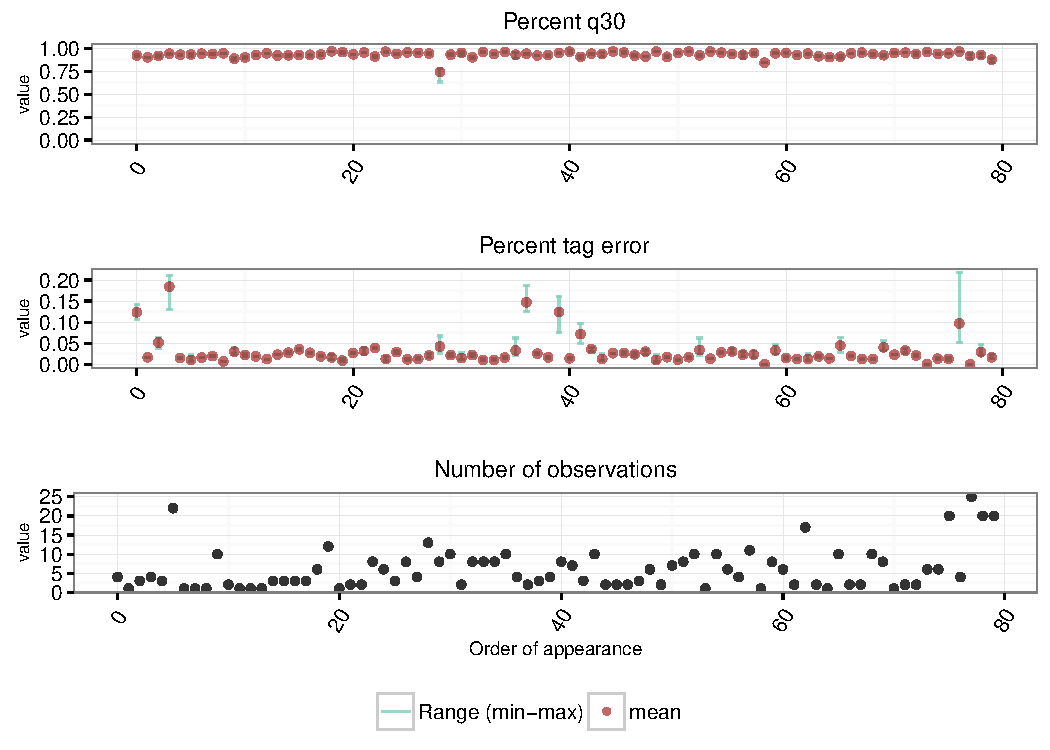
\includegraphics[width=\maxwidth]{figure/HiSeq6Comb-1} \caption[Figure showing the range (min to max) and mean of each succsessive run (flowcell) in lane 1, read 1, of the two variables Percent q30 and Percentage tag error]{Figure showing the range (min to max) and mean of each succsessive run (flowcell) in lane 1, read 1, of the two variables Percent q30 and Percentage tag error. All runs shown where performed on 126 cycles.}\label{fig:HiSeq6Comb}
\end{figure}

\begin{kframe}\begin{alltt}
\hlkwd{rm}\hlstd{(p1,p2,p3)}
\end{alltt}
\end{kframe}
\end{knitrout}
We will now investigate what we called the read level measurements. At this level only one observation per read and lane is supplied. We can therefore consider each run as a realisation of a random vector following a multivariate distribution. In this setting we have 7 different variables, with 16 measurements in each. Since the HiSeq 6 machine has been our main interest so far, we will continue in this fashion and compare it to the other HiSeq machines. All runs will henceforth be using all 8 lanes and a cycle setting on 126. The HiSeq 3 machine do not have any runs on this specific cycle setting and will therefore be omitted.

In Figure \ref{fig:MeanVectorFigure} we have the mean together with the range of the error rate variable. We can see that no measurements are zero in this case. The HiSeq 5 machine seems to have a consistently lower error rate compared to the other machines. The HiSeq 6 machine has shown one, or possibly several, runs with large error rates in different lanes. To further investigate the distribution of the error rate together with those variables which have not been looked upon, we will look at them in a histogram.  
\begin{knitrout}
\definecolor{shadecolor}{rgb}{0.969, 0.969, 0.969}\color{fgcolor}\begin{kframe}
\begin{alltt}
\hlcom{# Extract HiSeq 4 data on wide format. Remove rapid runs and then select error rate.}
\hlstd{Hiseq4} \hlkwb{<-} \hlkwd{ExtractBotLvlTimeseries}\hlstd{(}\hlkwd{c}\hlstd{(}\hlstr{"error_rate"}\hlstd{),}\hlstr{"HiSeq 4"}\hlstd{,All.df.reduced)} \hlopt
  \hlkwd{filter}\hlstd{(cycles}\hlopt{>=}\hlstd{Cycl[}\hlnum{1}\hlstd{],}
         \hlstd{cycles}\hlopt{<=}\hlstd{Cycl[}\hlnum{2}\hlstd{])} \hlopt
  \hlcom{# now remove those corresponding to rapid runs on the same cycle level, these only use 2 lanes and have NA on the rest}
  \hlkwd{na.omit}\hlstd{()} \hlopt
  \hlcom{# select error rate variable for each lane and read}
  \hlkwd{select}\hlstd{(}\hlkwd{grep}\hlstd{(}\hlstr{"error_rate"}\hlstd{,} \hlkwd{colnames}\hlstd{(.)))}
\hlcom{# Create Mean, max, min for each lane and read.}
\hlstd{Hiseq4} \hlkwb{<-} \hlkwd{data.frame}\hlstd{(}\hlstr{"Mean"}\hlstd{=}\hlkwd{colMeans}\hlstd{(Hiseq4),}
                     \hlstr{"Max"}\hlstd{=}\hlkwd{apply}\hlstd{(Hiseq4,}\hlnum{2}\hlstd{, max),}
                     \hlstr{"Min"}\hlstd{=}\hlkwd{apply}\hlstd{(Hiseq4,}\hlnum{2}\hlstd{, min),}
                     \hlstr{"lane_read"}\hlstd{=}\hlkwd{as.factor}\hlstd{(}\hlkwd{colnames}\hlstd{(Hiseq4)),}
                     \hlstr{"Machine"}\hlstd{=}\hlkwd{as.factor}\hlstd{(}\hlstr{"HiSeq 4"}\hlstd{))} \hlopt
  \hlcom{# place into long format for plotting}
  \hlkwd{melt}\hlstd{(}\hlkwc{measure.vars}\hlstd{=}\hlkwd{c}\hlstd{(}\hlstr{"Mean"}\hlstd{))}

\hlcom{# Do the same for HiSeq 5 data}
\hlstd{Hiseq5} \hlkwb{<-} \hlkwd{ExtractBotLvlTimeseries}\hlstd{(}\hlkwd{c}\hlstd{(}\hlstr{"error_rate"}\hlstd{),}\hlstr{"HiSeq 5"}\hlstd{,All.df.reduced)} \hlopt
    \hlkwd{filter}\hlstd{(cycles}\hlopt{>=}\hlstd{Cycl[}\hlnum{1}\hlstd{],}
           \hlstd{cycles}\hlopt{<=}\hlstd{Cycl[}\hlnum{2}\hlstd{])} \hlopt
   \hlkwd{na.omit}\hlstd{()} \hlopt
   \hlkwd{select}\hlstd{(}\hlkwd{grep}\hlstd{(}\hlstr{"error_rate"}\hlstd{,} \hlkwd{colnames}\hlstd{(.)))}

\hlstd{Hiseq5} \hlkwb{<-} \hlkwd{data.frame}\hlstd{(}\hlstr{"Mean"}\hlstd{=}\hlkwd{colMeans}\hlstd{(Hiseq5),}
                     \hlstr{"Max"}\hlstd{=}\hlkwd{apply}\hlstd{(Hiseq5,}\hlnum{2}\hlstd{, max),}
                     \hlstr{"Min"}\hlstd{=}\hlkwd{apply}\hlstd{(Hiseq5,}\hlnum{2}\hlstd{, min),}
                     \hlstr{"lane_read"}\hlstd{=}\hlkwd{as.factor}\hlstd{(}\hlkwd{colnames}\hlstd{(Hiseq5)),}
                     \hlstr{"Machine"}\hlstd{=}\hlkwd{as.factor}\hlstd{(}\hlstr{"HiSeq 5"}\hlstd{))} \hlopt
  \hlkwd{melt}\hlstd{(}\hlkwc{measure.vars}\hlstd{=}\hlkwd{c}\hlstd{(}\hlstr{"Mean"}\hlstd{))}

\hlcom{# Do the same for HiSeq 6 data}
\hlstd{Hiseq6} \hlkwb{<-} \hlkwd{ExtractBotLvlTimeseries}\hlstd{(}\hlkwd{c}\hlstd{(}\hlstr{"error_rate"}\hlstd{),}\hlstr{"HiSeq 6"}\hlstd{,All.df.reduced)} \hlopt
  \hlkwd{filter}\hlstd{(cycles}\hlopt{>=}\hlstd{Cycl[}\hlnum{1}\hlstd{],}
         \hlstd{cycles}\hlopt{<=}\hlstd{Cycl[}\hlnum{2}\hlstd{])} \hlopt
  \hlcom{# now remove those corresponding to rapid runs on the same cycle level, these only use 2 lanes and have NA on the rest}
  \hlkwd{na.omit}\hlstd{()} \hlopt
  \hlkwd{select}\hlstd{(}\hlkwd{grep}\hlstd{(}\hlstr{"error_rate"}\hlstd{,} \hlkwd{colnames}\hlstd{(.)))}

\hlstd{Hiseq6} \hlkwb{<-} \hlkwd{data.frame}\hlstd{(}\hlstr{"Mean"}\hlstd{=}\hlkwd{colMeans}\hlstd{(Hiseq6),}
                     \hlstr{"Max"}\hlstd{=}\hlkwd{apply}\hlstd{(Hiseq6,}\hlnum{2}\hlstd{, max),}
                     \hlstr{"Min"}\hlstd{=}\hlkwd{apply}\hlstd{(Hiseq6,}\hlnum{2}\hlstd{, min),}
                     \hlstr{"lane_read"}\hlstd{=}\hlkwd{as.factor}\hlstd{(}\hlkwd{colnames}\hlstd{(Hiseq6)),}
                     \hlstr{"Machine"}\hlstd{=}\hlkwd{as.factor}\hlstd{(}\hlstr{"HiSeq 6"}\hlstd{))} \hlopt
  \hlkwd{melt}\hlstd{(}\hlkwc{measure.vars}\hlstd{=}\hlkwd{c}\hlstd{(}\hlstr{"Mean"}\hlstd{))}

\hlstd{ggplot.tmp} \hlkwb{<-} \hlkwd{rbind}\hlstd{(Hiseq4,Hiseq5,Hiseq6)}
\hlkwd{levels}\hlstd{(ggplot.tmp}\hlopt{$}\hlstd{lane_read)} \hlkwb{<-} \hlkwd{do.call}\hlstd{(}\hlstr{"rbind"}\hlstd{,}\hlkwd{strsplit}\hlstd{(}\hlkwd{levels}\hlstd{(ggplot.tmp}\hlopt{$}\hlstd{lane_read),}\hlstr{"error_rate_"}\hlstd{))[,}\hlnum{2}\hlstd{]}

\hlcom{# Create mean and range figure for error rate.}
\hlkwd{ggplot}\hlstd{(ggplot.tmp,}
       \hlkwd{aes}\hlstd{(}\hlkwc{y}\hlstd{=value,} \hlkwc{x}\hlstd{=lane_read,} \hlkwc{color}\hlstd{=Machine))} \hlopt{+}
  \hlkwd{geom_point}\hlstd{(}\hlkwd{aes}\hlstd{(}\hlkwc{fill}\hlstd{=}\hlkwd{as.factor}\hlstd{(}\hlnum{1}\hlstd{)),} \hlkwc{size}\hlstd{=}\hlnum{2}\hlstd{,} \hlkwc{position}\hlstd{=}\hlkwd{position_dodge}\hlstd{(}\hlkwc{width}\hlstd{=}\hlnum{0.5}\hlstd{),} \hlkwc{alpha}\hlstd{=}\hlnum{0.8}\hlstd{)} \hlopt{+}
  \hlkwd{geom_errorbar}\hlstd{(}\hlkwd{aes}\hlstd{(}\hlkwc{ymax}\hlstd{=Max,} \hlkwc{ymin}\hlstd{=Min,} \hlkwc{width}\hlstd{=}\hlnum{0.2}\hlstd{,} \hlkwc{fill}\hlstd{=}\hlkwd{as.factor}\hlstd{(}\hlnum{2}\hlstd{)),} \hlkwc{alpha}\hlstd{=}\hlnum{0.5}\hlstd{,} \hlkwc{position}\hlstd{=}\hlkwd{position_dodge}\hlstd{(}\hlkwc{width}\hlstd{=}\hlnum{0.5}\hlstd{),} \hlkwc{show.legend} \hlstd{=} \hlnum{TRUE}\hlstd{)} \hlopt{+}
  \hlkwd{scale_y_continuous}\hlstd{(}\hlkwc{limits}\hlstd{=}\hlkwd{c}\hlstd{(}\hlopt{-}\hlnum{0.01}\hlstd{,}\hlnum{2}\hlstd{),} \hlkwc{breaks} \hlstd{=} \hlkwd{c}\hlstd{(}\hlnum{0}\hlstd{,}\hlnum{0.5}\hlstd{,}\hlnum{1}\hlstd{,}\hlnum{1.5}\hlstd{,}\hlnum{2}\hlstd{))} \hlopt{+}
  \hlkwd{coord_flip}\hlstd{()} \hlopt{+}
  \hlkwd{theme_bw}\hlstd{()} \hlopt{+}
  \hlkwd{scale_color_brewer}\hlstd{(}\hlkwc{type} \hlstd{=} \hlstr{"qual"}\hlstd{,} \hlkwc{palette}\hlstd{=}\hlnum{6}\hlstd{,}\hlkwc{guide} \hlstd{=} \hlkwd{guide_legend}\hlstd{(}\hlkwc{reverse}\hlstd{=}\hlnum{TRUE}\hlstd{))} \hlopt{+}
  \hlkwd{scale_fill_manual}\hlstd{(}\hlstr{""}\hlstd{,}
                    \hlkwc{labels}\hlstd{=}\hlkwd{c}\hlstd{(}\hlstr{"Mean"}\hlstd{,}\hlstr{"Range (min-max)"}\hlstd{),}
                    \hlkwc{values} \hlstd{=}\hlkwd{c}\hlstd{(}\hlstr{"black"}\hlstd{,}\hlstr{"blue"}\hlstd{))} \hlopt{+}
  \hlkwd{guides}\hlstd{(}\hlkwc{fill}\hlstd{=}\hlkwd{guide_legend}\hlstd{(}\hlkwc{override.aes}\hlstd{=}\hlkwd{list}\hlstd{(}\hlkwc{shape}\hlstd{=}\hlkwd{c}\hlstd{(}\hlnum{16}\hlstd{,}\hlnum{NA}\hlstd{),} \hlkwc{linetype}\hlstd{=}\hlkwd{c}\hlstd{(}\hlnum{0}\hlstd{,}\hlnum{1}\hlstd{))))} \hlopt{+}
  \hlkwd{xlab}\hlstd{(}\hlstr{"Error rate (lane_read)"}\hlstd{)}
\end{alltt}
\end{kframe}\begin{figure}[!htb]
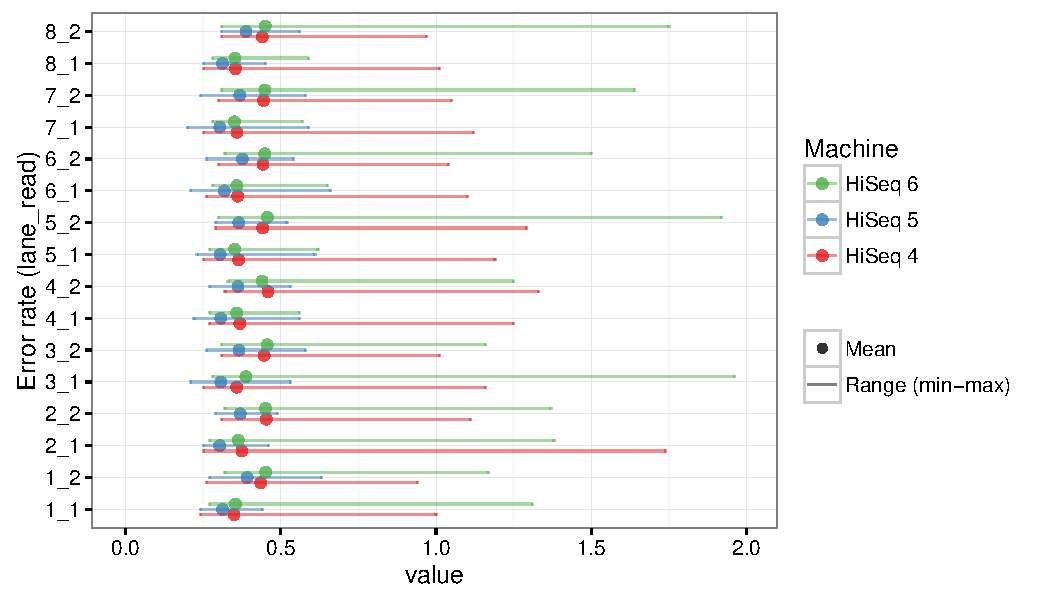
\includegraphics[width=\maxwidth]{figure/MeanVectorFigure-1} \caption[Mean together with the range of the error rate (read\_level) of each lane and read (lane\_read)]{Mean together with the range of the error rate (read\_level) of each lane and read (lane\_read). Notice that the HiSeq 5 has the lowest mean error rate of all HiSeq machines.}\label{fig:MeanVectorFigure}
\end{figure}


\end{knitrout}

\begin{knitrout}
\definecolor{shadecolor}{rgb}{0.969, 0.969, 0.969}\color{fgcolor}\begin{kframe}
\begin{alltt}
\hlcom{# Extract HiSeq 6 data, all variables on read level}
\hlstd{HiSeq6.botlvl.series} \hlkwb{<-} \hlkwd{ExtractBotLvlTimeseries}\hlstd{(}\hlkwd{c}\hlstd{(}\hlstr{"mean_q"}\hlstd{,}\hlstr{"pct_q30"}\hlstd{,}\hlstr{"error_rate"}\hlstd{,}\hlstr{"raw_clusters"}\hlstd{,}\hlstr{"raw_density"}\hlstd{,}\hlstr{"pf_clusters"}\hlstd{,}\hlstr{"pf_density"}\hlstd{),}\hlstr{"HiSeq 6"}\hlstd{,All.df.reduced)}
\hlcom{## Extract "High output v4" runs: 102-126 cycles using 8 lanes}
\hlstd{v4.HiSeq6.botlvl.series} \hlkwb{<-} \hlkwd{filter}\hlstd{(HiSeq6.botlvl.series,}
                                  \hlstd{cycles}\hlopt{>=}\hlstd{Cycl[}\hlnum{1}\hlstd{],}
                                  \hlstd{cycles}\hlopt{<=}\hlstd{Cycl[}\hlnum{2}\hlstd{])} \hlopt
  \hlcom{# now remove rapid runs on the same cycle level, these only use 2 lanes and have NA on the rest}
  \hlkwd{na.omit}\hlstd{()}
\end{alltt}
\end{kframe}
\end{knitrout}
In Figure \ref{fig:ReadlvlER} we have a histograms of the error rate, raw cluster density and the number of raw clusters for lane 1 and 2, both reads. In the error rate (row one), we can see that read 2 contains more variability compared to read 1. The distribution of read 1 is more peaked while the distribution for read 2 is quite flat. We can also see that the distribution is somewhat skewed, tending towards the right. For the two later rows, the density and cluster variable can be seen to be close to symmetric. The distribution of the density and cluster variables also look very much alike. 
%Error rate measurements from read 1 can be stable while read 2 deviates. An example can be seen around the 20th observation in the error rate for lane 1. 
%This deviating behaviour is not necessarily seen in any other variable, in the same lane and read. 
%What can be seen in the second and third row is that the raw- density and cluster variables correlate almost perfectly. 
%This is seen in several variables. The following variables is almost perfectly correlated; raw clusters, post filter clusters, raw density, post filter density for each read inside a lane. 
%We will exclude all but the raw clusters variable in the analysis. 
%The raw cluster variable is also almost perfectly correlated for each read inside a lane. This can be seen in Figure \ref{fig:ReadlvlER} when comparing the variables inbetween reads for a given lane. 
%We will remove read 2 for the raw cluster variable in every lane, from the analysis.  
\begin{knitrout}
\definecolor{shadecolor}{rgb}{0.969, 0.969, 0.969}\color{fgcolor}\begin{kframe}
\begin{alltt}
\hlcom{# Code found online and has been slightly modified.}
\hlcom{# http://stackoverflow.com/questions/11610377/how-do-i-change-the-formatting-of-numbers-on-an-axis-with-ggplot}
\hlstd{fancy_printing} \hlkwb{<-} \hlkwa{function}\hlstd{(}\hlkwc{l}\hlstd{) \{}
     \hlcom{# turn in to character string in scientific notation}
     \hlstd{l} \hlkwb{<-} \hlkwd{format}\hlstd{(l,} \hlkwc{scientific} \hlstd{=} \hlnum{TRUE}\hlstd{)}
     \hlkwa{for} \hlstd{(i} \hlkwa{in} \hlnum{1}\hlopt{:}\hlkwd{length}\hlstd{(l))\{}
       \hlkwa{if} \hlstd{(}\hlkwd{grepl}\hlstd{(}\hlstr{"NA"}\hlstd{,l[i])}\hlopt{==}\hlnum{TRUE}\hlstd{)\{}
         \hlstd{l[i]} \hlkwb{<-} \hlstd{l[i]}
       \hlstd{\}}\hlkwa{else}\hlstd{\{}
         \hlkwa{if} \hlstd{(}\hlkwd{as.numeric}\hlstd{(l[i])}\hlopt{>}\hlnum{2}\hlstd{)\{}
           \hlcom{# quote the part before the exponent to keep all the digits}
           \hlstd{l[i]} \hlkwb{<-} \hlkwd{gsub}\hlstd{(}\hlstr{"^(.*)e"}\hlstd{,} \hlstr{"'\textbackslash{}\textbackslash{}1'e"}\hlstd{, l[i])}
           \hlcom{# turn the 'e+' into plotmath format}
           \hlstd{l[i]} \hlkwb{<-} \hlkwd{gsub}\hlstd{(}\hlstr{"e"}\hlstd{,} \hlstr{"%.%10^"}\hlstd{, l[i])}
         \hlstd{\}}\hlkwa{else}\hlstd{\{}
          \hlstd{l[i]} \hlkwb{<-} \hlkwd{as.numeric}\hlstd{(l[i])}
         \hlstd{\}}
       \hlstd{\}}
     \hlstd{\}}
     \hlcom{# return this as an expression}
     \hlkwd{parse}\hlstd{(}\hlkwc{text}\hlstd{=l)}
\hlstd{\}}
\hlcom{#fancy_printing(c("   NA","1e8"))}
\hlkwd{ggplot}\hlstd{(}\hlkwd{melt}\hlstd{(}
  \hlkwd{select}\hlstd{(v4.HiSeq6.botlvl.series,}
    \hlkwd{starts_with}\hlstd{(}\hlstr{"error_rate_1"}\hlstd{),}
    \hlkwd{starts_with}\hlstd{(}\hlstr{"error_rate_2"}\hlstd{),}
    \hlkwd{starts_with}\hlstd{(}\hlstr{"raw_density_1"}\hlstd{),}
    \hlkwd{starts_with}\hlstd{(}\hlstr{"raw_density_2"}\hlstd{),}
    \hlkwd{starts_with}\hlstd{(}\hlstr{"raw_clusters_1"}\hlstd{),}
    \hlkwd{starts_with}\hlstd{(}\hlstr{"raw_clusters_2"}\hlstd{),}
    \hlstd{Date),}
  \hlkwc{id.vars}\hlstd{=}\hlstr{"Date"}\hlstd{),}
  \hlkwd{aes}\hlstd{(}\hlkwc{x}\hlstd{=value))} \hlopt{+}
  \hlkwd{geom_histogram}\hlstd{()} \hlopt{+}
  \hlkwd{facet_wrap}\hlstd{(}\hlstr{"variable"}\hlstd{,} \hlkwc{scales} \hlstd{=} \hlstr{"free_x"}\hlstd{,}\hlkwc{ncol}\hlstd{=}\hlnum{4}\hlstd{)} \hlopt{+}
  \hlkwd{theme_bw}\hlstd{()} \hlopt{+}
  \hlkwd{theme}\hlstd{(}\hlkwc{legend.position}\hlstd{=}\hlstr{"none"}\hlstd{,} \hlkwc{plot.margin}\hlstd{=}\hlkwd{unit}\hlstd{(}\hlkwd{c}\hlstd{(}\hlnum{5.5}\hlstd{,} \hlnum{15}\hlstd{,} \hlnum{5.5}\hlstd{,} \hlnum{5.5}\hlstd{),}\hlstr{"points"}\hlstd{))}  \hlopt{+}
  \hlkwd{scale_x_continuous}\hlstd{(}\hlkwc{breaks}\hlstd{=scales}\hlopt{::}\hlkwd{pretty_breaks}\hlstd{(}\hlkwc{n}\hlstd{=}\hlnum{3}\hlstd{),} \hlkwc{labels}\hlstd{=fancy_printing)}
\end{alltt}


{\ttfamily\noindent\itshape\color{messagecolor}{\#\# `stat\_bin()` using `bins = 30`. Pick better value with `binwidth`.}}\end{kframe}\begin{figure}[!htb]
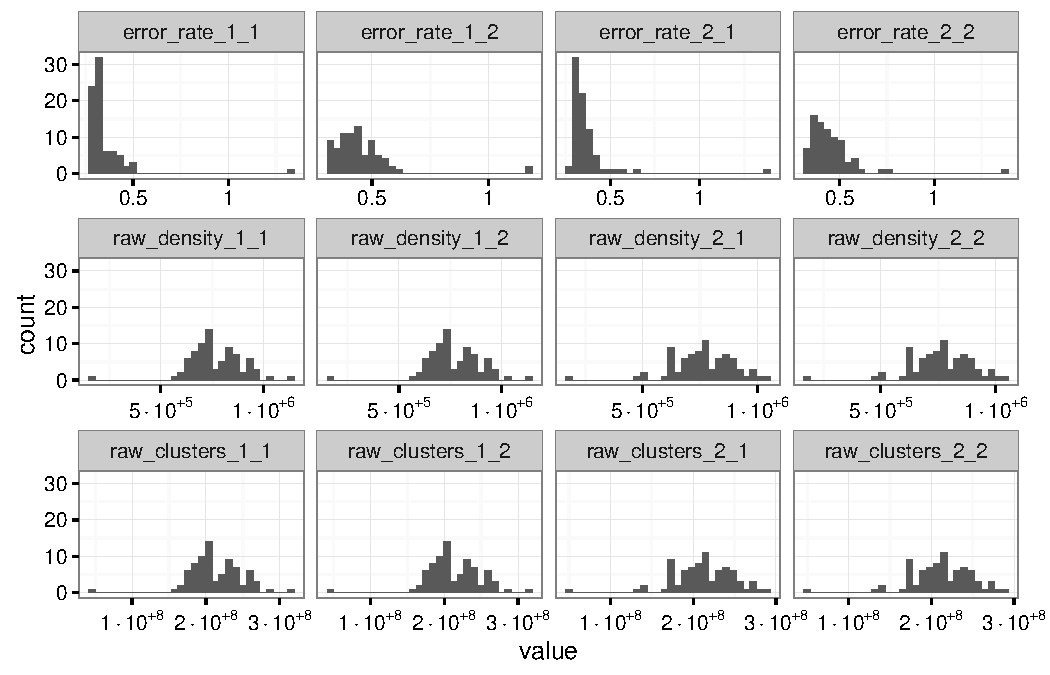
\includegraphics[width=\maxwidth]{figure/ReadlvlER-1} \caption[Error rates, the raw density and the number of raw clusters for each read in lanes 1 and 2]{Error rates, the raw density and the number of raw clusters for each read in lanes 1 and 2. The variable name are listed in the following manner: Variable\_lane\_read.}\label{fig:ReadlvlER}
\end{figure}


\end{knitrout}
The Spearman correlation matrix is visualized in Figure \ref{fig:ReadlvlCor}. The number of variables in the Figure is equal to $112$. The correlation matrix is estimated from a sample size of $79$. In this figure the axis labels where omitted but a header for each group of variables is placed next to them. As an example, the top 16 variables in Figure \ref{fig:ReadlvlCor} corresponds to the error rate for each read and lane which is denoted by the label. We will refer to this as a section of variables. 

We can see that the density and cluster sections of variables correlate almost perfectly. This is especially true for measurements on the same read in a lane. The mean q and percent q30 sections seem to be correlated to each other while not having much correlation to the cluster and density variables. The error rate is negatively correlated with percent q30 and mean q measurements from the same read and lane, while not showing much correlation to other reads and lanes. The correlation matrix can almost be placed on a block diagonal form where three first sections of variables create one block and the last four create another. %Variables on the same read and lane seem to be correlated well while 
%A deviating pattern is is also seen in this section of variables. Those mean q and percent q30 corresponding to lane 7 read 1 and 2, shows much less correlation to the variables inside and outside section but shows very strong correlation to eachother. Also, the percent tag error shows correlation between lanes with low lane number (\textit{reformulate?}) but lanes with high lane number show very little correlation to the others. 

For further analysis we will consider the quality control data for HiSeq 6 with variables mean q, error rate and percent q30. We will continue to use a cycle setting of 126. The mean q, error rate can be assumed to have support on the positive real line. These variables can not be assumed to follow a normal distribution and will therefore be transformed. We will use a Box-Cox transformation (cf. \citet{BoxCox}) on these variables and estimate the transformation parameter $\lambda$ using the Guerro method (cf. \citet{Gurrero}). Also, if necessary, we will divide the transformed variables by a constant to change the scale. The percent q30 variable has limited support on $(0,1)$ and will be transformed using the quantile normal function. Before the transformation and estimation of transformation parameters are performed we will remove those runs which are poor. Runs will be classified as poor using todays quality control criterias. 

The transformation methods are more thoroughly presented in the Appendix, section \ref{NormalSection}. In this section, we also assess the assumption of normality for the transformed HiSeq 6 data, for the variables previously mentioned, together with the a short investigation of autocorrelation. For further analysis, we assume that the transformed data of the mean q, error rate and percent q30 variables are generated by a multivariate normal distribution. 
\begin{knitrout}
\definecolor{shadecolor}{rgb}{0.969, 0.969, 0.969}\color{fgcolor}\begin{kframe}
\begin{alltt}
\hlstd{ggp} \hlkwb{<-} \hlkwd{VizCor}\hlstd{(v4.HiSeq6.botlvl.series[,}\hlopt{-}\hlkwd{c}\hlstd{(}\hlnum{1}\hlopt{:}\hlnum{3}\hlstd{)],} \hlkwc{method}\hlstd{=}\hlstr{"spearman"}\hlstd{,}\hlkwc{title}\hlstd{=}\hlstr{""}\hlstd{)}
\hlstd{N} \hlkwb{<-} \hlkwd{ncol}\hlstd{(v4.HiSeq6.botlvl.series)}

\hlstd{tmpFUN} \hlkwb{<-} \hlkwa{function}\hlstd{(}\hlkwc{x}\hlstd{)} \hlkwd{return} \hlstd{(}\hlkwd{cbind}\hlstd{(}\hlkwd{c}\hlstd{(}\hlnum{2}\hlopt{+}\hlnum{8}\hlopt{*}\hlstd{(}\hlnum{1}\hlopt{+}\hlnum{2}\hlopt{*}\hlstd{x)),}\hlkwd{c}\hlstd{(N}\hlopt{-}\hlnum{8}\hlopt{*}\hlstd{(}\hlnum{1}\hlopt{+}\hlnum{2}\hlopt{*}\hlstd{x))))}
\hlstd{df.tmp} \hlkwb{<-} \hlkwd{tmpFUN}\hlstd{(}\hlkwd{seq}\hlstd{(}\hlnum{0}\hlstd{,}\hlnum{6}\hlstd{))}

\hlstd{df.tmp} \hlkwb{<-} \hlkwd{data.frame}\hlstd{(}\hlkwc{TEXT}\hlstd{=}\hlkwd{c}\hlstd{(}\hlstr{"Error rate"}\hlstd{,}\hlstr{"Mean Q"}\hlstd{,}\hlstr{"Percent q30"}\hlstd{,}\hlstr{"PF clusters"}\hlstd{,}\hlstr{"PF density"}\hlstd{,}\hlstr{"Raw clusters"}\hlstd{,}\hlstr{"Raw density"}\hlstd{),df.tmp)}

\hlstd{ggp} \hlkwb{<-} \hlstd{ggp} \hlopt{+}
   \hlkwd{theme}\hlstd{(}\hlkwc{axis.text.x} \hlstd{=} \hlkwd{element_blank}\hlstd{(),}
          \hlkwc{axis.text.y} \hlstd{=} \hlkwd{element_blank}\hlstd{())}

\hlcom{# add text to picture}
\hlkwa{for} \hlstd{(i} \hlkwa{in} \hlnum{1}\hlopt{:}\hlkwd{nrow}\hlstd{(df.tmp))\{}
  \hlstd{ggp} \hlkwb{<-} \hlstd{ggp} \hlopt{+}
   \hlkwd{geom_text}\hlstd{(}\hlkwc{x}\hlstd{=df.tmp[i,}\hlnum{2}\hlstd{],} \hlkwc{y}\hlstd{=df.tmp[i,}\hlnum{3}\hlstd{],}\hlkwc{label}\hlstd{=df.tmp[i,}\hlnum{1}\hlstd{],}
             \hlkwc{angle}\hlstd{=}\hlopt{-}\hlnum{45}\hlstd{,}\hlkwc{size}\hlstd{=}\hlnum{3.2}\hlstd{,}\hlkwc{family}\hlstd{=}\hlstr{"Times"}\hlstd{)}
\hlstd{\}}
\hlstd{tmpFUN} \hlkwb{<-} \hlkwa{function}\hlstd{(}\hlkwc{x}\hlstd{)} \hlkwd{return}\hlstd{(}\hlkwd{cbind}\hlstd{(N}\hlopt{-}\hlstd{(}\hlnum{2}\hlopt{+}\hlnum{16}\hlopt{*}\hlstd{x)}\hlopt{-}\hlnum{1}\hlopt{/}\hlnum{2}\hlstd{,}\hlnum{16}\hlopt{*}\hlstd{x}\hlopt{+}\hlnum{1}\hlopt{/}\hlnum{2}\hlstd{))}
\hlstd{df.tmp} \hlkwb{<-} \hlkwd{tmpFUN}\hlstd{(}\hlnum{1}\hlopt{:}\hlnum{7}\hlstd{)} \hlopt \hlkwd{as.data.frame}\hlstd{()}
\hlcom{# Draw lines to create sections}
\hlkwa{for} \hlstd{(i} \hlkwa{in} \hlnum{1}\hlopt{:}\hlkwd{nrow}\hlstd{(df.tmp))\{}
  \hlstd{ggp} \hlkwb{<-} \hlstd{ggp} \hlopt{+}
    \hlkwd{geom_segment}\hlstd{(}\hlkwc{y}\hlstd{=df.tmp[i,}\hlnum{1}\hlstd{],} \hlkwc{x}\hlstd{=}\hlnum{0.5}\hlstd{,} \hlkwc{xend}\hlstd{=df.tmp[i,}\hlnum{2}\hlstd{],} \hlkwc{yend}\hlstd{=df.tmp[i,}\hlnum{1}\hlstd{],} \hlkwc{color}\hlstd{=}\hlstr{"#0000004D"}\hlstd{,} \hlkwc{size}\hlstd{=}\hlnum{0.2}\hlstd{)} \hlopt{+}
    \hlkwd{geom_segment}\hlstd{(}\hlkwc{x}\hlstd{=df.tmp[i,}\hlnum{1}\hlstd{],} \hlkwc{y}\hlstd{=}\hlnum{0.5}\hlstd{,} \hlkwc{xend}\hlstd{=df.tmp[i,}\hlnum{1}\hlstd{],} \hlkwc{yend}\hlstd{=df.tmp[i,}\hlnum{2}\hlstd{],} \hlkwc{color}\hlstd{=}\hlstr{"#0000004D"}\hlstd{,} \hlkwc{size}\hlstd{=}\hlnum{0.2}\hlstd{)}
\hlstd{\}}
\hlcom{# print}
\hlstd{ggp}
\end{alltt}
\end{kframe}\begin{figure}
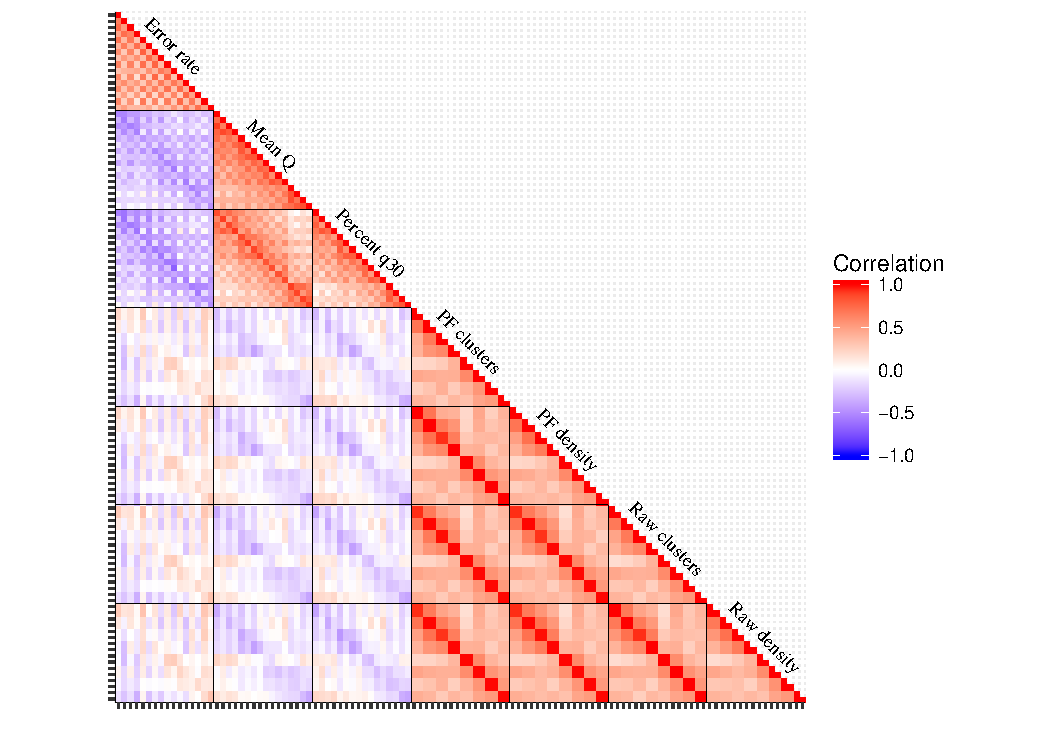
\includegraphics[width=\maxwidth]{figure/ReadlvlCor-1} \caption[Spearman correlation matrix of HiSeq 6 Read level measurements]{Spearman correlation matrix of HiSeq 6 Read level measurements. Two groupings can be seen in the correlation.}\label{fig:ReadlvlCor}
\end{figure}

\begin{kframe}\begin{alltt}
\hlcom{# remove}
\hlkwd{rm}\hlstd{(df.tmp, tmpFUN)}
\end{alltt}
\end{kframe}
\end{knitrout}


\begin{knitrout}
\definecolor{shadecolor}{rgb}{0.969, 0.969, 0.969}\color{fgcolor}\begin{kframe}
\begin{alltt}
\hlcom{# Create a IC sample by removing values runs with large error rates and low pf_clusters}
\hlstd{Hiseq6.tag} \hlkwb{<-}
  \hlkwd{filter}\hlstd{(df.sample.results,}
         \hlstd{Instrument} \hlopt{==} \hlstr{"HiSeq 6"}\hlstd{,}
         \hlstd{cycles} \hlopt{<} \hlstd{Cycl[}\hlnum{2}\hlstd{],}
         \hlstd{cycles} \hlopt{>} \hlstd{Cycl[}\hlnum{1}\hlstd{])}

\hlstd{Hiseq6.read} \hlkwb{<-} \hlkwd{filter}\hlstd{(All.df.reduced,}
                      \hlstd{Instrument}\hlopt{==}\hlstr{"HiSeq 6"}\hlstd{,}
                      \hlstd{cycles} \hlopt{<} \hlstd{Cycl[}\hlnum{2}\hlstd{],}
                      \hlstd{cycles} \hlopt{>} \hlstd{Cycl[}\hlnum{1}\hlstd{])}
\hlcom{# function which creates a IC sample.}
\hlstd{CreateICsample} \hlkwb{<-} \hlkwa{function}\hlstd{(}\hlkwc{x}\hlstd{,} \hlkwc{y}\hlstd{,}\hlkwc{quality_crit}\hlstd{)\{}
  \hlcom{# x : (data.frame) data from tag level}
  \hlcom{# y : (data.frame) data from read level}
  \hlcom{# quality_crit: (list) what are quality criteras which are going to be used to create this IC sample.}
  \hlcom{# Example: list(err=..., pct_q30=...)}

  \hlkwd{library}\hlstd{(dplyr)}
  \hlstd{IC.read} \hlkwb{<-} \hlstd{y} \hlopt
    \hlkwd{filter}\hlstd{(error_rate} \hlopt{<} \hlstd{quality_crit}\hlopt{$}\hlstd{err,}
           \hlstd{pf_clusters} \hlopt{>} \hlstd{quality_crit}\hlopt{$}\hlstd{pf_clusters)}

  \hlcom{# How many flowcells are removed?}
  \hlcom{# FlowcellRemoved <- anti_join(IC.read,y,by="flowcell_id")$flowcell_id %>% unique() }

  \hlcom{# Remove flowcells which are not ok to the quality characteristics}
  \hlstd{Data} \hlkwb{<-} \hlkwd{semi_join}\hlstd{(x,IC.read,}\hlkwc{by}\hlstd{=}\hlstr{"flowcell_id"}\hlstd{)}

  \hlkwd{return}\hlstd{(}\hlkwd{list}\hlstd{(}\hlkwc{IC.tag} \hlstd{= Data,}
              \hlkwc{IC.read} \hlstd{= IC.read))}
\hlstd{\}}

\hlstd{IC.Hiseq6.sample} \hlkwb{<-} \hlkwd{CreateICsample}\hlstd{(}\hlkwc{x}\hlstd{=Hiseq6.tag,}
                                   \hlkwc{y}\hlstd{=Hiseq6.read,}
                                   \hlkwc{quality_crit} \hlstd{=} \hlkwd{list}\hlstd{(}\hlkwc{err}\hlstd{=}\hlnum{1}\hlstd{,}
                                                       \hlkwc{pf_clusters}\hlstd{=}\hlnum{1e8}\hlstd{))}

\hlstd{IC.Hiseq6} \hlkwb{<-} \hlkwd{ExtractBotLvlTimeseries}\hlstd{(}\hlkwd{c}\hlstd{(}\hlstr{"mean_q"}\hlstd{,}\hlstr{"pct_q30"}\hlstd{,}\hlstr{"error_rate"}\hlstd{),}
                                     \hlkwc{machine}\hlstd{=}\hlstr{"HiSeq 6"}\hlstd{,}
                                     \hlkwc{Data}\hlstd{=}\hlkwd{group_by}\hlstd{(IC.Hiseq6.sample}\hlopt{$}\hlstd{IC.read))} \hlopt
  \hlkwd{na.omit}\hlstd{()}

\hlkwd{rm}\hlstd{(df.sample.results,All.df.reduced,HiSeq6.botlvl.series,Hiseq6.tag,Hiseq6.read,Missing,All.nas)}
\end{alltt}


{\ttfamily\noindent\color{warningcolor}{\#\# Warning in rm(df.sample.results, All.df.reduced, HiSeq6.botlvl.series, Hiseq6.tag, : object 'All.nas' not found}}\end{kframe}
\end{knitrout}

\begin{knitrout}
\definecolor{shadecolor}{rgb}{0.969, 0.969, 0.969}\color{fgcolor}\begin{kframe}
\begin{alltt}
\hlstd{TransformDataFun} \hlkwb{<-} \hlkwa{function}\hlstd{(}\hlkwc{x}\hlstd{)\{}
  \hlstd{lambda} \hlkwb{<-} \hlstd{forecast}\hlopt{::}\hlkwd{BoxCox.lambda}\hlstd{(x);}
  \hlkwd{return}\hlstd{(}\hlkwd{list}\hlstd{(}\hlkwc{Lambda}\hlstd{=lambda,}
              \hlkwc{data}\hlstd{=forecast}\hlopt{::}\hlkwd{BoxCox}\hlstd{(x,lambda)))}
\hlstd{\}}
\hlstd{colnam} \hlkwb{<-} \hlkwd{colnames}\hlstd{(IC.Hiseq6[,}\hlopt{-}\hlkwd{c}\hlstd{(}\hlnum{1}\hlopt{:}\hlnum{3}\hlstd{)])}
\hlstd{PCT} \hlkwb{<-} \hlkwd{grep}\hlstd{(}\hlstr{"pct"}\hlstd{,colnam)}

\hlstd{TransformedData} \hlkwb{<-} \hlstd{IC.Hiseq6[,}\hlopt{-}\hlkwd{c}\hlstd{(}\hlnum{1}\hlopt{:}\hlnum{3}\hlstd{)]}

\hlstd{TransformedData.tmp} \hlkwb{<-} \hlkwd{apply}\hlstd{(TransformedData[,}\hlopt{!}\hlnum{1}\hlopt{:}\hlkwd{ncol}\hlstd{(TransformedData)} \hlopt \hlstd{PCT],} \hlnum{2}\hlstd{, TransformDataFun)}

\hlstd{Lambdas} \hlkwb{<-} \hlkwd{lapply}\hlstd{(TransformedData.tmp,}\hlkwa{function}\hlstd{(}\hlkwc{x}\hlstd{) x}\hlopt{$}\hlstd{Lambda)} \hlopt \hlkwd{unlist}\hlstd{()}

\hlstd{TransformedData.tmp} \hlkwb{<-} \hlkwd{lapply}\hlstd{(TransformedData.tmp,} \hlkwa{function}\hlstd{(}\hlkwc{x}\hlstd{) x}\hlopt{$}\hlstd{data)} \hlopt \hlkwd{do.call}\hlstd{(}\hlstr{"cbind"}\hlstd{,.)}

\hlstd{TransformedData[,}\hlopt{!}\hlnum{1}\hlopt{:}\hlkwd{ncol}\hlstd{(TransformedData)} \hlopt \hlstd{PCT]} \hlkwb{<-} \hlstd{TransformedData.tmp}
\hlcom{# Transform with quantile function}
\hlstd{TransformedData[,PCT]} \hlkwb{<-} \hlkwd{apply}\hlstd{(TransformedData[,}\hlnum{1}\hlopt{:}\hlkwd{ncol}\hlstd{(TransformedData)} \hlopt \hlstd{PCT],}\hlnum{2}\hlstd{,}\hlkwa{function}\hlstd{(}\hlkwc{x}\hlstd{)} \hlkwd{qnorm}\hlstd{(x))}
\hlcom{#save(TransformedData, file="../Data/ICdata.Rdata")}
\end{alltt}
\end{kframe}
\end{knitrout}

\begin{knitrout}
\definecolor{shadecolor}{rgb}{0.969, 0.969, 0.969}\color{fgcolor}\begin{kframe}
\begin{alltt}
\hlstd{K} \hlkwb{<-} \hlnum{100}
\hlstd{OrgOrder} \hlkwb{<-} \hlkwd{colnames}\hlstd{(TransformedData)}
\hlcom{# divide by a constant!}
\hlstd{TransformedData[,}\hlnum{1}\hlopt{:}\hlkwd{ncol}\hlstd{(TransformedData)} \hlopt \hlkwd{grep}\hlstd{(}\hlstr{"mean"}\hlstd{,OrgOrder)]} \hlkwb{<-} \hlstd{TransformedData[,}\hlnum{1}\hlopt{:}\hlkwd{ncol}\hlstd{(TransformedData)} \hlopt \hlkwd{grep}\hlstd{(}\hlstr{"mean"}\hlstd{,OrgOrder)]}\hlopt{/}\hlstd{K}

\hlstd{t2} \hlkwb{<-} \hlstd{MVN}\hlopt{::}\hlkwd{hzTest}\hlstd{(TransformedData)}
\end{alltt}


{\ttfamily\noindent\itshape\color{messagecolor}{\#\# sROC 0.1-2 loaded}}\begin{alltt}
\hlstd{t4} \hlkwb{<-} \hlstd{mvShapiroTest}\hlopt{::}\hlkwd{mvShapiro.Test}\hlstd{(}\hlkwd{as.matrix}\hlstd{(TransformedData))}
\hlcom{#save(Lambdas,t2,t4,file = "../Data/LambdaAndXtable.Rdata")}
\end{alltt}
\end{kframe}
\end{knitrout}





\bibliography{REFERENCES.bib}
\end{document}
